% This is based on the LLNCS.DEM the demonstration file of
% the LaTeX macro package from Springer-Verlag
% for Lecture Notes in Computer Science,
% version 2.4 for LaTeX2e as of 16. April 2010
%
% See http://www.springer.com/computer/lncs/lncs+authors?SGWID=0-40209-0-0-0
% for the full guidelines.
%
\documentclass{llncs}

\usepackage{graphicx}
\graphicspath{ {images/} }
\usepackage{float}

\begin{document}

\title{Informational Analysis of Monte Carlo Simulations of Spin Systems}
%
%\titlerunning{Hamiltonian Mechanics}  % abbreviated title (for running head)
%                                     also used for the TOC unless
%                                     \toctitle is used
%
\author{Galina Malovichko}
%
%\authorrunning{Ivar Ekeland et al.} % abbreviated author list (for running head)
%
%%%% list of authors for the TOC (use if author list has to be modified)
%\tocauthor{Ivar Ekeland, Roger Temam, Jeffrey Dean, David Grove,
%Craig Chambers, Kim B. Bruce, and Elisa Bertino}
%
\institute{University of California, Davis\\
\email{gmalovichko@ucdavis.edu} } %,\\ WWW home page:
%\texttt{http://users/\homedir iekeland/web/welcome.html}
%\and
%Universit\'{e} de Paris-Sud,
%Laboratoire d'Analyse Num\'{e}rique, B\^{a}timent 425,\\
%F-91405 Orsay Cedex, France}

\maketitle              % typeset the title of the contribution

\begin{abstract}
The Monte-Carlo Simulation of simplest nearest-neighbour Ising model was ran on four different spin systems. Random spin flipping on each step of the simulation was used to create sequence of 0s (spin does not flip) and 1s (spin does not flip). Entropy rate of these sequences was then compared to thermodynamic entropy of the systems and showed strong similarity to it.
%\keywords{computational geometry, graph theory, Hamilton cycles}
\end{abstract}
%
\section{Monte Carlo simulation of Ising Model}
%
Systems of spins can be described with different Hamiltonian models. Ising model is one of the simplest and most popular of such models.
In Ising systems, spins are sitting in the nodes of the regular lattice and assume values $S_i = \pm 1$. Energy of the magnetic interactions between the spins is given by the expression:

\begin{equation}
 H = -J \sum_{\langle i, j \rangle}{S_i S_j}\\
 \label{eq:one}
\end{equation}

\begin{figure}
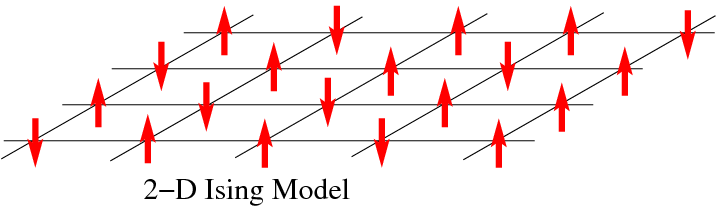
\includegraphics[width=0.8\linewidth]{ising.png}
\centering
\end{figure}

Summation here is taken over all pairs of nearest neighbours in the lattice. In ferromagnetics coupling $J$ is positive, so at low temperatures, when total energy of the system is small, all spins are aligned. As temperature increases, thermal fluctuations make them disordered.

A spin can change its orientation and the likelihood of this change depends on energy gain associated with the change and temperature of the system. At each step of Monte Carlo simulation we choose a random spin and flip it with certain probability. Different algorithms use different expressions for probability. 

In my simulation I used "heat bath" update algorithm that follows following steps:

\begin{itemize}
\item Flip random spin
\item Find energy change $\Delta E$, associated with this flip.
\item Keep the spin flipped with probability $p = \frac{1}{1 + \exp{\frac{\Delta E}{T}}}$
\end{itemize}

The lattice is usually initialized with randomly oriented spins and periodic boundary conditions, then updated enough times (I used 4000 $\times$ size of the lattice updates) to bring it to thermal equilibrium at a given temperature. This initial stage is called "thermalization".

After it is over, we can update the system further, measuring its energy, magnetization and other thermodynamic properties after each update and averaging them to find their means. I used 10000 $\times$ size of the lattice updates to do these measurements.

This figure shows average energy of several 2D lattices in $J$ units as function of temperature. At zero temperature all spins are aligned and energy per site is $-J \cdot (\mbox{number of nearest neighbours}) / 2 = -2 J$. As the temperature grows, spins become disordered ant total energy approaches zero.

\begin{figure}[h!]
\includegraphics[width=0.8\linewidth]{2D__E_vs_T.png}
\centering
\end{figure}

\begin{figure}[H]
\includegraphics[width=0.8\linewidth]{2D__M_vs_T.png}
\centering
\end{figure}

Magnetization, that is equal to absolute sum of all spins, divided by the size of the lattice, also depends on the temperature. It equals to one at zero temperature and zero as high temperature.


We are particularly interested in the entropy of the system. It can be calculates as the integral

\begin{equation}
S(\beta) = E \beta - \int_0^{\beta} E d\beta\\
\end{equation}

where $\beta = \frac{1}{T}$. Normalized by the size of the lattice, entropy equals to zero when all spins are ordered and approaches one at high temperatures when each spin is equally likely to be oriented up or down. Notice that to find entropy at a given temperature $T$ we need to measure $E(T)$ for all temperatures larger than $T$ to perform numerical integration.

\begin{figure}[h]
\includegraphics[width=0.8\linewidth]{2D__S_vs_T.png}
\centering
\end{figure}

The whole spin lattice can in principle be described with binary alphabet, for example ascribing symbol 1 to spin up and 0 to spin down, but the information analysis of such system, having two spacial dimensions and evolving in time, can be complicated.
We would like our simulation to produce a binary string that we would be able to run information analysis on.
I used the spin flips string as such string: on every step of Monte Carlo simulation, if the spin was flipped, I appended 1 to this string. If the spin kept its orientation, I appended 0.

Then I ran Bayesian analysis on this string of 0s and 1s and acquired entropy rate at each temperature for square lattice of $8 \times 8$ spins. Plots of thermodynamic entropy and of entropy rate look remarkably similar.

It is not surprising for them to approach the same values in the limiting cases of $T \to 0$ or $T \to \infty$. At zero temperature all spins keep their orientation, so the simulation produces sequence of all zeroes, which has zero entropy rate.
At high temperatures, spins flip independently of their neighbours, with $1/2$ probability. Simulation generates sequence of zeroes and ones that is equivalent to the output of fair coin. Such sequence has entropy rate of 1.

\begin{figure}[h!]
\includegraphics[width=0.8\linewidth]{2D__hmu_and_S_vs_T.png}
\centering
\end{figure}

The surprising part of the plot is how (relatively) well two curves agree between these two limiting cases. Thermodynamic entropy seems to be systematically lower than informational entropy rate, but that might be explained by underestimated integral in the entropy expression. I obviously cannot integrate numerically all the way to $T = \infty$, so the upper tail of the integral is cut short.

First of all, it is remarkable that global entropy of the system, that depends only on model Hamiltonian and configuration of the lattice matches so well entropy rate of the local updates of the lattice state. It would be interesting to investigate the theory behind this match and explain it analytically.

If we can indeed prove and show that for different lattices thermodynamical entropy can be approximated with entropy rate of flips sequence (perhaps, with some necessary adjustments and normalizations), it would make entropy measurement much faster. We would no longer need to measure $E(T)$ on the whole interval $[T, \infty)$, single simulation at the temperature of interest would be enough.


%
\section{Different lattices}
%
While mathematical proof of the equivalence of two entropies might be too ambitious goal for this small project, running the simulation on different lattices and comparing thermodynamical entropy and entropy rate in each case is definitely doable.

I investigated three other lattices in addition to previously shown 2D. They are all square lattices, all described with the same Hamiltonian (\ref{eq:one}) and only differ in their dimensions.

\begin{figure}[h!]
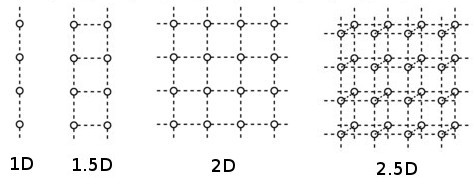
\includegraphics[width=0.8\linewidth]{lattices.jpg}
\centering
\end{figure}

1D lattice is just a chain of spins, with two neighbours for each spin. Ladder (also called 1.5D) and bilayer (also called 2.5D) are special cases, which can exhibit both properties of higher and lower dimensional lattices.

I ran Monte Carlo simulation on all four lattices and acquired their energies and magnetizations as functions of temperature. Energy at zero temperature is negative and proportional to the number of nearest neighbours (or coordination number) of each lattice. Magnetization starts at 1 at zero temperature and becomes zero as temperature increases. Notice that transition temperature is different for different lattices.

\begin{figure}[H]
\includegraphics[width=0.8\linewidth]{all__E_vs_T.png}
\includegraphics[width=0.8\linewidth]{all__M_vs_T.png}
\includegraphics[width=0.8\linewidth]{all__hmu_and_S_vs_T.png}
\centering
\end{figure}

Like before, the most interesting thermodynamical quantity in these simulations is entropy and its relationship to entropy rate of the spin flips sequence.

The third image on the previous page shows simulated thermodynamical entropies (colored lines) and entropy rates of spin flips (black lines).
The lines seem to be in good, though not perfect, agreement.


%
\section{Critical temperature}
%
Both condensed matter theorists and experimentalists are interested in the phase transition between ferro- and paramagnetic states of the spin system. Second order transition is characterized by singularities in the second derivative of the free energy at so called critical temperature(temperature of the phase transition).

Heat capacity and magnetic susceptibility are examples of such derivatives and both of them show peaks near critical temperature (vertical grey line) for 2D lattice. We observe finite peaks rather than singularities because the system has finite size.

\begin{figure}[H]
\includegraphics[width=0.7\linewidth]{2D__C_vs_T.png}
\includegraphics[width=0.7\linewidth]{2D__X_vs_T.png}
\centering
\end{figure}

% \begin{figure}[H]

% \centering
% \end{figure}

Vladimir Iglovikov in project "Information and Order Parameters in the Gauge Ising Model" for Natural Computation and Self-Organization class in Spring 2014 has found another quantity that peaks at critical temperature: excess entropy or shared information between the past and the future of spin flips string.

Unfortunately, I failed to reproduce this result: Bayesian inference algorithm modeled the $\epsilon$-machine that generated 0s and 1s sequence as a biased coin with only one state and zero excess entropy. Only at very low temperatures, when the fraction of 1s in the sequence was less than a few percent, Bayesian machine did sometimes have more than one state. I am unsure whether this result is reliable.


\begin{figure}[H]
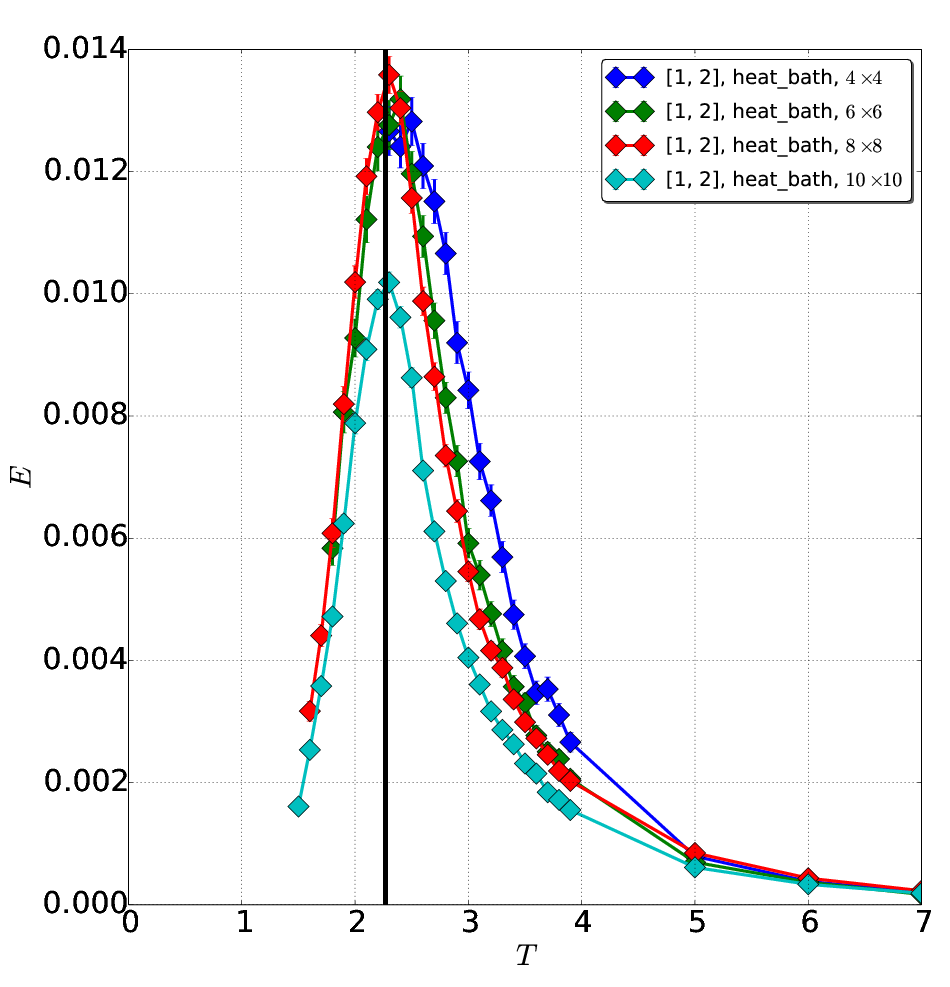
\includegraphics[width=0.55\linewidth]{vlad.png}
\centering
\end{figure}

%
\section{Future development}
%
I have already raised some points that might be interesting to look at in the future and I am going to list them again:

\begin{itemize}
\item Can the relationship between thermodynamical entropy and entropy rate of the spin flips be proven mathematically?

\item Would this relationship hold for other spin systems, such as 3D lattices, hexagonal lattices, systems with continuous spins or systems, described with more complicated Hamiltonian?

\item Can we use other symbol strings for similar purposes? For example, string of states of a given spin rather than string of random spin flips? Will the result differ?

\item Can the results be useful for computing entropy? Will informational analysis save computation time?

\end{itemize}


\end{document}
